\documentclass{mimosis}

\usepackage{metalogo}

%%%%%%%%%%%%%%%%%%%%%%%%%%%%%%%%%%%%%%%%%%%%%%%%%%%%%%%%%%%%%%%%%%%%%%%%
% Some of my favourite personal adjustments
%%%%%%%%%%%%%%%%%%%%%%%%%%%%%%%%%%%%%%%%%%%%%%%%%%%%%%%%%%%%%%%%%%%%%%%%
%
% These are the adjustments that I consider necessary for typesetting
% a nice thesis. However, they are *not* included in the template, as
% I do not want to force you to use them.

% This ensures that I am able to typeset bold font in table while still aligning the numbers
% correctly.
\usepackage{etoolbox}
\usepackage{lipsum}
\usepackage{subcaption}
\usepackage{amsfonts}

\usepackage{color}
\definecolor{myred}{rgb}{0.8588,0.2667,0.2157}
\newcommand{\TODO}[1]{\color{myred} \textbf{#1} \color{black}}
\renewcommand{\vec}[1]{\ensuremath{\mathbf{#1}}} % vectors

\usepackage[binary-units=true]{siunitx}
\DeclareSIUnit\px{px}

\sisetup{%
  detect-all           = true,
  detect-family        = true,
  detect-mode          = true,
  detect-shape         = true,
  detect-weight        = true,
  detect-inline-weight = math,
}

%%%%%%%%%%%%%%%%%%%%%%%%%%%%%%%%%%%%%%%%%%%%%%%%%%%%%%%%%%%%%%%%%%%%%%%%
% Hyperlinks & bookmarks
%%%%%%%%%%%%%%%%%%%%%%%%%%%%%%%%%%%%%%%%%%%%%%%%%%%%%%%%%%%%%%%%%%%%%%%%

\usepackage[%
  colorlinks = true,
  citecolor  = RoyalBlue,
  linkcolor  = RoyalBlue,
  urlcolor   = RoyalBlue,
  ]{hyperref}

\usepackage{bookmark}

%%%%%%%%%%%%%%%%%%%%%%%%%%%%%%%%%%%%%%%%%%%%%%%%%%%%%%%%%%%%%%%%%%%%%%%%
% Bibliography
%%%%%%%%%%%%%%%%%%%%%%%%%%%%%%%%%%%%%%%%%%%%%%%%%%%%%%%%%%%%%%%%%%%%%%%%
%
% I like the bibliography to be extremely plain, showing only a numeric
% identifier and citing everything in simple brackets. The first names,
% if present, will be initialized. DOIs and URLs will be preserved.

\usepackage[%
  autocite     = plain,
  backend      = bibtex,
  doi          = true,
  url          = true,
  giveninits   = true,
  hyperref     = true,
  maxbibnames  = 99,
  maxcitenames = 99,
  sortcites    = true,
  style        = numeric,
  ]{biblatex}

%%%%%%%%%%%%%%%%%%%%%%%%%%%%%%%%%%%%%%%%%%%%%%%%%%%%%%%%%%%%%%%%%%%%%%%%
% Some adjustments to make the bibliography more clean
%%%%%%%%%%%%%%%%%%%%%%%%%%%%%%%%%%%%%%%%%%%%%%%%%%%%%%%%%%%%%%%%%%%%%%%%
%
% The subsequent commands do the following:
%  - Removing the month field from the bibliography
%  - Fixing the Oxford commma
%  - Suppress the "in" for journal articles
%  - Remove the parentheses of the year in an article
%  - Delimit volume and issue of an article by a colon ":" instead of
%    a dot ""
%  - Use commas to separate the location of publishers from their name
%  - Remove the abbreviation for technical reports
%  - Display the label of bibliographic entries without brackets in the
%    bibliography
%  - Ensure that DOIs are followed by a non-breakable space
%  - Use hair spaces between initials of authors
%  - Make the font size of citations smaller
%  - Fixing ordinal numbers (1st, 2nd, 3rd, and so) on by using
%    superscripts

% Remove the month field from the bibliography. It does not serve a good
% purpose, I guess. And often, it cannot be used because the journals
% have some crazy issue policies.
\AtEveryBibitem{\clearfield{month}}
\AtEveryCitekey{\clearfield{month}}

% Fixing the Oxford comma. Not sure whether this is the proper solution.
% More information is available under [1] and [2].
%
% [1] http://tex.stackexchange.com/questions/97712/biblatex-apa-style-is-missing-a-comma-in-the-references-why
% [2] http://tex.stackexchange.com/questions/44048/use-et-al-in-biblatex-custom-style
%
\AtBeginBibliography{%
  \renewcommand*{\finalnamedelim}{%
    \ifthenelse{\value{listcount} > 2}{%
      \addcomma
      \addspace
      \bibstring{and}%
    }{%
      \addspace
      \bibstring{and}%
    }
  }
}

% Suppress "in" for journal articles. This is unnecessary in my opinion
% because the journal title is typeset in italics anyway.
\renewbibmacro{in:}{%
  \ifentrytype{article}
  {%
  }%
  % else
  {%
    \printtext{\bibstring{in}\intitlepunct}%
  }%
}

% Remove the parentheses for the year in an article. This removes a lot
% of undesired parentheses in the bibliography, thereby improving the
% readability. Moreover, it makes the look of the bibliography more
% consistent.
\renewbibmacro*{issue+date}{%
  \setunit{\addcomma\space}
    \iffieldundef{issue}
      {\usebibmacro{date}}
      {\printfield{issue}%
       \setunit*{\addspace}%
       \usebibmacro{date}}%
  \newunit}

% Delimit the volume and the number of an article by a colon instead of
% by a dot, which I consider to be more readable.
\renewbibmacro*{volume+number+eid}{%
  \printfield{volume}%
  \setunit*{\addcolon}%
  \printfield{number}%
  \setunit{\addcomma\space}%
  \printfield{eid}%
}

% Do not use a colon for the publisher location. Instead, connect
% publisher, location, and date via commas.
\renewbibmacro*{publisher+location+date}{%
  \printlist{publisher}%
  \setunit*{\addcomma\space}%
  \printlist{location}%
  \setunit*{\addcomma\space}%
  \usebibmacro{date}%
  \newunit%
}

% Ditto for other entry types.
\renewbibmacro*{organization+location+date}{%
  \printlist{location}%
  \setunit*{\addcomma\space}%
  \printlist{organization}%
  \setunit*{\addcomma\space}%
  \usebibmacro{date}%
  \newunit%
}

% Display the label of a bibliographic entry in bare style, without any
% brackets. I like this more than the default.
%
% Note that this is *really* the proper and official way of doing this.
\DeclareFieldFormat{labelnumberwidth}{#1\adddot}

% Ensure that DOIs are followed by a non-breakable space.
\DeclareFieldFormat{doi}{%
  \mkbibacro{DOI}\addcolon\addnbspace
    \ifhyperref
      {\href{http://dx.doi.org/#1}{\nolinkurl{#1}}}
      %
      {\nolinkurl{#1}}
}

% Use proper hair spaces between initials as suggested by Bringhurst and
% others.
\renewcommand*\bibinitdelim {\addnbthinspace}
\renewcommand*\bibnamedelima{\addnbthinspace}
\renewcommand*\bibnamedelimb{\addnbthinspace}
\renewcommand*\bibnamedelimi{\addnbthinspace}

% Make the font size of citations smaller. Depending on your selected
% font, you might not need this.
\renewcommand*{\citesetup}{%
  \biburlsetup
  \small
}

\DeclareLanguageMapping{english}{english-mimosis}

\addbibresource{report.bib}

%%%%%%%%%%%%%%%%%%%%%%%%%%%%%%%%%%%%%%%%%%%%%%%%%%%%%%%%%%%%%%%%%%%%%%%%
% Fonts
%%%%%%%%%%%%%%%%%%%%%%%%%%%%%%%%%%%%%%%%%%%%%%%%%%%%%%%%%%%%%%%%%%%%%%%%

\ifxetexorluatex
  \setmainfont{Minion Pro}
\else
  \usepackage[lf]{ebgaramond}
  \usepackage[oldstyle,scale=0.7]{sourcecodepro}
  \singlespacing
\fi

\renewcommand{\th}{\textsuperscript{\textup{th}}\xspace}

\makeindex
\makeglossaries

%%%%%%%%%%%%%%%%%%%%%%%%%%%%%%%%%%%%%%%%%%%%%%%%%%%%%%%%%%%%%%%%%%%%%%%%
% Incipit
%%%%%%%%%%%%%%%%%%%%%%%%%%%%%%%%%%%%%%%%%%%%%%%%%%%%%%%%%%%%%%%%%%%%%%%%

\title{\texttt{RGBD-Slam from RGB Smartphone Video}}
\subtitle{Project report for the summer course of 3D Computer Vision 2020}
\author{Peter Hügel and Florian Fallenbüchel}

\begin{document}
  \frontmatter

  \sloppy
  \begin{titlepage}
  \vspace*{5cm}
  \makeatletter
  \begin{center}
    \begin{Huge}
      \@title
    \end{Huge}\\[0.1cm]
    %
    \begin{Large}
      \@subtitle
    \end{Large}\\
    %
    \emph{by}\\
    \@author
  \end{center}
  \makeatother
\end{titlepage}


  % \include{sources/abstract}

  \tableofcontents

  \mainmatter
  \sloppy

  \chapter{Introduction}
    Our idea for the 3D Computer Vision mini project was to create high quality 3D reconstructions from regular smartphone videos, without the need for an expensive RGB-D camera like the Microsoft Kinect.
    To make this feasible, we try to combine fine-tuned depth map estimates from Convolutional Neural Networks (CNNs) with state of the art RGBD-SLAM methods.\\
    For the estimation of the depth maps we rely on the approach of Luo et al. \cite{luo2020consistent} (Consistent Video Depth Estimation) to fine-tune the monocular depth estimation model from Google, which was initially trained on the Mannequin Challenge dataset \cite{mannequin}.
    Their method addresses the usual problems of monocular depth estimation and promises to produce plausible, geometrically and temporally consistent depth maps for any input video, which is a key element for high-quality reconstructions.
    This method provides us with our depth estimates, as well as relatively accurate camera extrinsics and intrinsics. which are obtained from bundle adjustment of sparse SIFT points using COLMAP \cite{colmap}.\\
    These are the initial values for our reconstruction approach, which is strongly based on the Bundle Fusion paper \cite{dai2017bundlefusion}.
    Dai et al. are proposing a two-step (sparse then dense) pose optimization with a strong focus on real-time applicability.
    Since the fine-tuning of the depth estimates cannot be done in real-time, we are only interested in their optimization strategies.
    More specific, we only apply their fine-scaled dense optimization strategy for pixel-level alignment of the frames, since their hierarchical sparse optimization has the primary focus of real-time applicability, and does not yield higher accuracy than our exhaustively matched points aquired from COLMAP.
    Finally we integrate the data into a scalable truncated signed distance function (TSDF) voxel volume with the optimized camera trajectory using Open3D \cite{open3d}. Open3D gives us some handy features and allows us to easily extract textured meshes from these volumes for visualization.


  \chapter{Method}
    Our idea was to apply the method from \citetitle{luo2020consistent}~\cite{luo2020consistent} to fine-tune a CNN and use the refined depth estimates as well as the inherently produced COLMAP camera in- and extrinsics for 3D reconstructions.
    Before reconstructing, we wanted to improve the initial pose estimates from COLMAP with an energy minimization approach in the fashion of \citetitle{dai2017bundlefusion}~\cite{dai2017bundlefusion}.

    \section{Depth Estimation}
        The geometric loss proposed in \citetitle{luo2020consistent} already requires a lot of geometric information of the scene, which is also required for 3D reconstruction.
        Luo et al. use COLMAP to extract SIFT points from every frame of the input video and then match these points exhaustively to calculate precise camera parameters for the entire scene.
        They then create accurate masks of optical flow between two frames through forward-backward consistency check of FlowNet estimates.
        If enough pixels are valid, a pair of frames is used for training.
        During training, they project the depth estimates of one frame to the coordinate frame of the other image and compare it with the values of that prediction at the positions given through the optical flow masks.
        The loss is comprised of two parts, spatial and disparity loss.
        The spatial loss is the difference between the target pixel position through projection and the position from FlowNet.
        The disparity loss gives the absolute distance between the z-components of the two depth vectors in a common 3D camera space.
        They combine these losses and backpropagate them through the depth estimation network.
        Since the camera in- and extrinsics, as well as the flow masks, are fixed for the fine-tuning, the only way for the model to reduce this error is to produce depth maps which result in basically unique points in the common global coordinate frame for this input.
        They use every consecutive frame pair for training, resulting in temporal consistency, but also more distant pairs in a hierarchical manner, for higher geometric consistency.\\
        To make the depth maps of the CNN comparable to the extrinsics produced by COLMAP, they have to calibrate the relative scale.
        In order to do this, they let COLMAP produce semi-dense depth estimates from the sparse reconstruction results and compute the difference in ratio to the CNN for every frame.
        They then simply divide the camera translations by the mean of the scales to bring the extrinsics into the range of the initial CNN depth maps.\\
        This brings us to our first problem with the realization of the consistent depth maps.
        For the calibration of the scale, they invert the semi-dense COLMAP depth map by simply doing $inv\_cmp\_dpt = 1 / cmp\_dpt$ in their code.
        During execution, this lead to cases where we encountered division by zero in the scale calibration.
        We believe that this made the training unstable, since we had the issue that the loss of the network sometimes became NaN during an epoch.
        We tried to fix this by adding a small $eps$ to the COLMAP depth maps and afterwards we did not encounter NaNs or division by zero anymore.\\
        We don't want to blame the issues entirely on this, since we did not do enough testing to rule out other possibilities, and since this did not fix our second issue with the consistent depth maps, namely holes in the predicted depth map at random locations (but consistent for the sequence).
        \begin{figure}
            \centering
            
\includegraphics[width=0.33\textwidth]{images/hole.png}
            
\includegraphics[width=0.33\textwidth]{images/hole_zoom.png}
            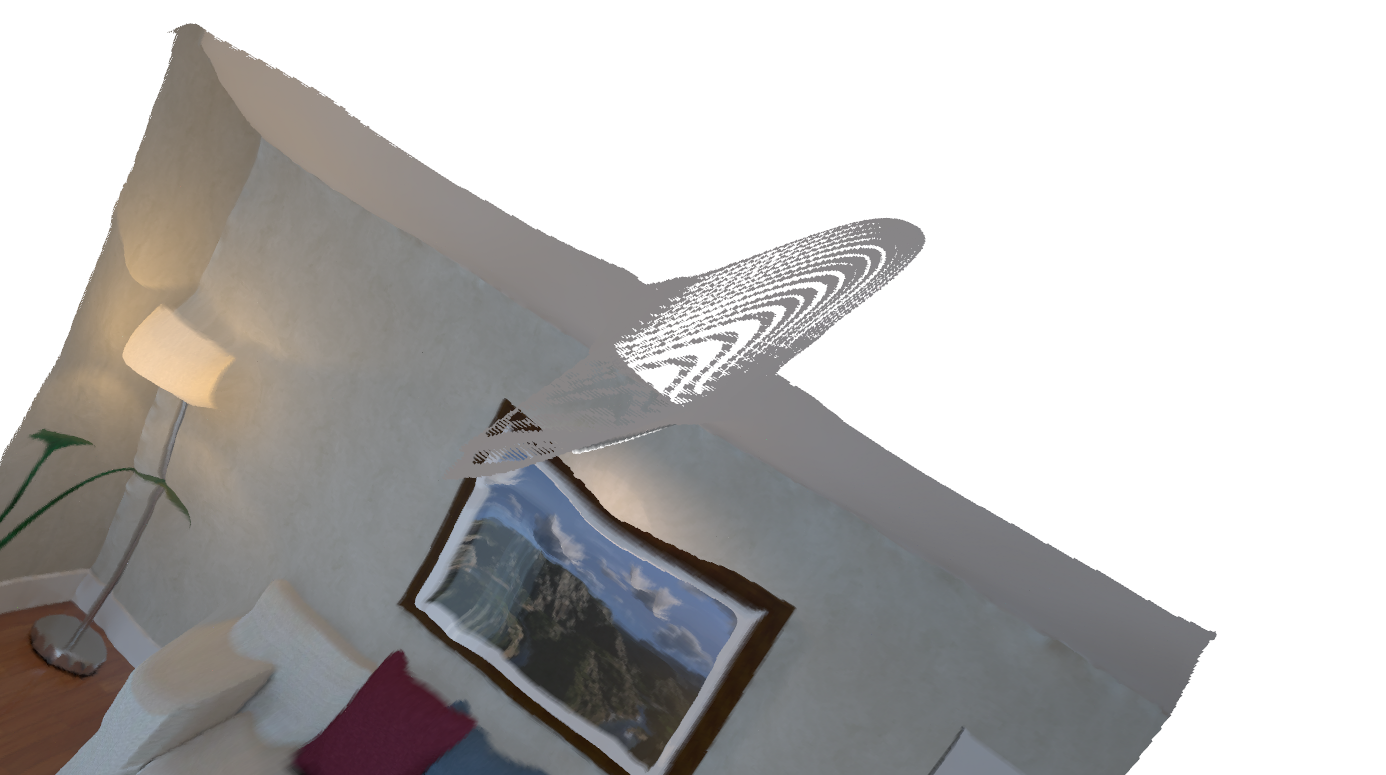
\includegraphics[width=0.33\textwidth]{images/hole_recon.png}
            \caption{Hole in the top corner of the image with basically infinite depth leads to huge deformations of the 3D reconstruction.}
            \label{holes}
        \end{figure}
        Figure~\ref{holes} shows an example of such a black hole present in the predictions for the ground truth dataset.
        These holes add a massive error to the reconstruction, influencing the scaling of the image and making consistent volume integration at these locations impossible.
        We have no idea what causes this problem and how we should counter it, leaving the depth maps from this approach flawed.
        We still use these results as well as the sparsely optimized COLMAP parameters for further optimization.
    
    \section{Pose Optimization}\label{sec:method_pose_optimization}
        Using the estimates for the depth and global pose from the previous step, we technically have everything for a 3D reconstruction.
        Before that we wanted to improve on the pose estimation by closely following the methods employed in \citetitle{dai2017bundlefusion}~\cite{dai2017bundlefusion}.
        The hierarchical structure they propose is required for their online reconstruction as it drastically reduces the computational requirements.
        As we aimed for an offline reconstruction, we were able to cut a few of the optimization steps they employed.\\
        Their method for the pose optimization contains a sparse part and a dense part.
        As the reconstruction progresses they reduce the weight of the sparse term and increase the weight of the dense term.
        Since we start with the sparse pose estimation from COLMAP and want to simply refine our poses, we ignore their sparse term and focus on the dense term.\\
        The optimization we implemented is formulated as an error minimization problem where the total dense error is the sum of the photometric and geometric error:
        \begin{equation}
            E_{\text{dense}}(X) = E_{\text{photo}}(X) + E_{\text{geo}}(X)
            \label{eq:edense}
        \end{equation}
        Where $X$ contains the global pose $T$ of every image.
        Both Terms are evaluated onover all valid image pairs.
        Two images are considered a valid image pair, two conditions are met.
        The camera angle difference between two frames has to be below a threshold that we ended up setting to 50\textdegree.
        The second requirement for an image pair is a minimum overlap of 20\%.
        A pixel is overlapping if it's 3D position lies within the view frustum of the other image.
        We precompute the image pairs and store them in a matrix $M$ of size $N \times N$ with $M(i,j) = 1$ if $i$ and $j$ form a valid image pair.\\
        The photometric term is based on the luminance gradient $I$, as it is more robust against lighting changes.
        \begin{equation}
            E_{\text{photo}}(X) =
            \frac{1}{v} \sum_{(i,j) | M(i,j)=1}\sum_{k=0}^{\left\lvert I_i \right\rvert}
            \left\lvert\left\lvert
            I_i(K^{-1}(d_{i,k})) - I_j(K^{-1}(T_j^{-1}T_id_{i,k}))
            \right\rvert\right\rvert_2^2
            \label{eq:ephoto}
        \end{equation}
        Where $K$ are the camera intrinsics, $d_{i,k}$ is the 3D position of the pixel $k$ in image $i$, and $v$ is the number of valid pixels that contributed to the error.
        For an image pair, pixels are valid if their 3D position lies within the view frustum of the other camera position.
        \begin{equation}
            E_{\text{geo}}(X) =
            \frac{1}{v} \sum_{(i,j) | M(i,j)=1}\sum_{k=0}^{\left\lvert D_i \right\rvert}
            \left[
            n_{i,k}^T \left(d_{i,k} - T_i^{-1}T_jK \left( D_j \left( K^{-1}\left( T_j^{-1}T_id_{i,k} \right) \right) \right)\right)
            \right]^2
            \label{eq:egeo}
        \end{equation}
        While $I_i(x,y)$ gives us the luminance gradient at an image coordinate $(x,y)$ within image $i$, $D_i(x,y)$ provides us with the depth at the specified pixel in image $i$.
        $n_{i,k}$ is the normal vector at pixel $k$ in image $i$, we compute the normals with open3d.\\
        We believe some further elaboration regarding equations~\ref{eq:ephoto} and \ref{eq:egeo} may be useful.
        For one, the left part of equation~\ref{eq:ephoto},
        \begin{equation*}
            I_i(K^{-1}(d_{i,k})),
        \end{equation*}
        is simply the luminance at pixel $k$ in image $i$.
        While $K^{-1}(d_{i,k})$ results in a 3d vector, the last dimension can be removed in order to obtain the pixel coordinates $x$ and $y$.
        Then $I_i(x,y)$ is essentially a function that maps the pixel coordinates to the 2d luminance gradient vector.
        For the right side of equation~\ref{eq:ephoto},
        \begin{equation*}
            I_j(K^{-1}(T_j^{-1}T_id_{i,k})),
        \end{equation*}
        we have to consider that $d_{i,k}$ is a 3d vector and the transforms $T_i$ and $T_j^{-1}$ are both $4 \times 4$ matrices.
        Therefore $d_{i,k}$ has to be expanded by one dimension by appending $1$ to it.
        It can then be transformed by $T_i$ and $T_j^{-1}$.
        Th resulting 4d vector has to be reduced to a 3d vector before the inverse intrinsics can be applied to it in order to obtain the pixel coordinate.\\
        For the purpose of understanding these terms we have visualized the following equation for an image pair $(i, j)$:
        \begin{equation}
            C_j(K^{-1}(T_j^{-1}T_id_{i,k})) \coloneqq C_i(K^{-1}d_{i,k})
            \label{eq:vis_perspective}
        \end{equation}
        The visualization of equation~\ref{eq:vis_perspective} can be seen in figure~\ref{fig:vis_perspective}.
        The combination of $T_j^{-1}T_i$ transforms the 3d point $d_{i,k}$ of image $i$ into the global pose of image $i$ and then out of the pose of image $j$.
        The combination is then simply the transform from image $i$ to image $j$.
        In other words, we look at the 3d point $d_{i,k}$ from the camera position of image $j$.
        With the inverse of the intrinsics matrix we retrieve the pixel coordinates that this point would fall into if viewed from the new position.
        For the visualization we write the color information of every pixel from image $i$ into the new pixel position in image $j$.
        All pixels in image $j$ that haven't been hit are set to zero.
        \begin{figure}[ht]
            \centering
            \begin{subfigure}[b]{.45\textwidth}
                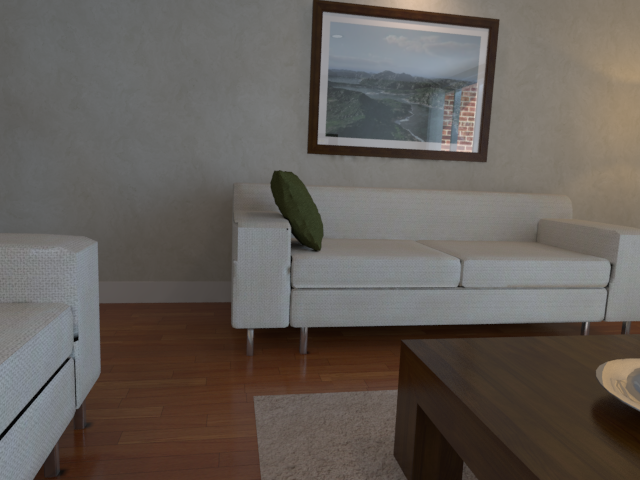
\includegraphics[width=.95\textwidth]{images/vis_perspective_01}
                \caption{original image $i$}
                \label{sfig:i_original}
            \end{subfigure}
            \begin{subfigure}[b]{.45\textwidth}
                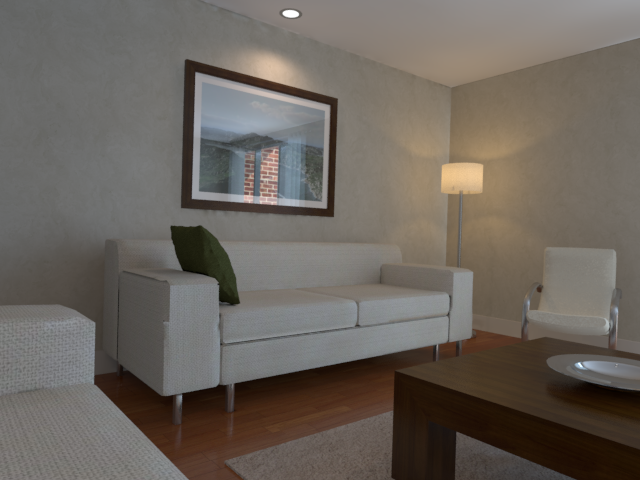
\includegraphics[width=.95\textwidth]{images/vis_perspective_03}
                \caption{original image $j$}
                \label{sfig:j_original}
            \end{subfigure}
            \begin{subfigure}[b]{.45\textwidth}
                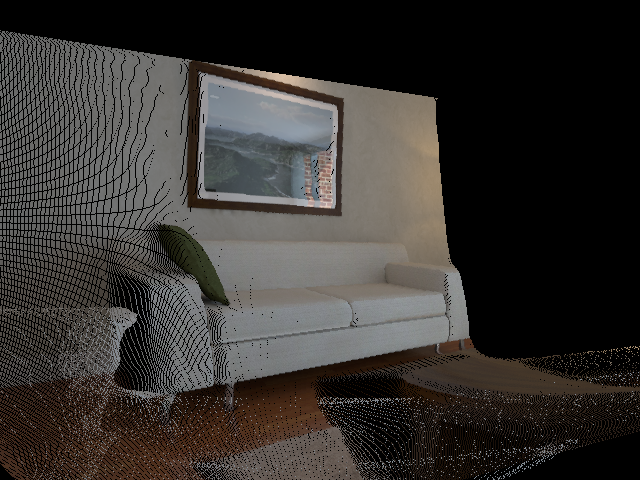
\includegraphics[width=.95\textwidth]{images/vis_perspective_02}
                \caption{information from image $i$ viewed from the camera position of image $j$}
                \label{sfig:i_from_j}
            \end{subfigure}
            \caption[]{Visual interpretation of what happens in the error terms $E_{\text{geo}}$ and $E_{\text{phoyo}}$, described through equation~\ref{eq:vis_perspective}}
            \label{fig:vis_perspective}
        \end{figure}
        In order to solve the minimization problem from equation~\ref{eq:edense} we use the function scipy.optimize.minimize.
        While this is a very inefficient and slow process, it manages to obtain a more fitting set of extrinsics according to our cost function.
        \todo{hier noch ueber unsere $d_{i,k}$ solution/precomputation reden! fand ich ziemlich comfy, dass das precomputable ist (bis auf den depth teil)}
    \section{3D Reconstruction}
        \todo{my reason to skip pose estimation for now is, that it is a bit of a story.\\
        1 get depth \& extrinsics\\
        2 use them\\
        3 improve on extrinsics.\\
        we tried out different approaches for the reconstruction and ended up using open3d\\
        talk about modifying the extrinsics to make everything work\\
        maybe talk about integration and deintegration (used by bundle fusion as it is live and they update their reconstruction)\\
        to improve on the shitty reconstruction we wanted to optimize the extrinsics. this would nicely lead into the next section!!!\\
        compare extrinsics to ground truth with the matlab 3d plot?}

  \chapter{Results}
    In this chapter we present our results for the implementation of our pose estimation and the depth map acquired from \citetitle{luo2020consistent}~\cite{luo2020consistent}.
    We try to pinpoint the problems we encountered in our pipeline by comparing our results to the synthetic dataset 'lr kt2' from \citetitle{handa:etal:ICRA2014}~\cite{handa:etal:ICRA2014}.
    \section{pose optimization}
        Figure~\ref{fig:initial_reconstruction} shows our first valid results for one of our own videos.
        We were hoping to drastically improve on this results after optimizing the global poses.
        \begin{figure}[ht]
            \centering
            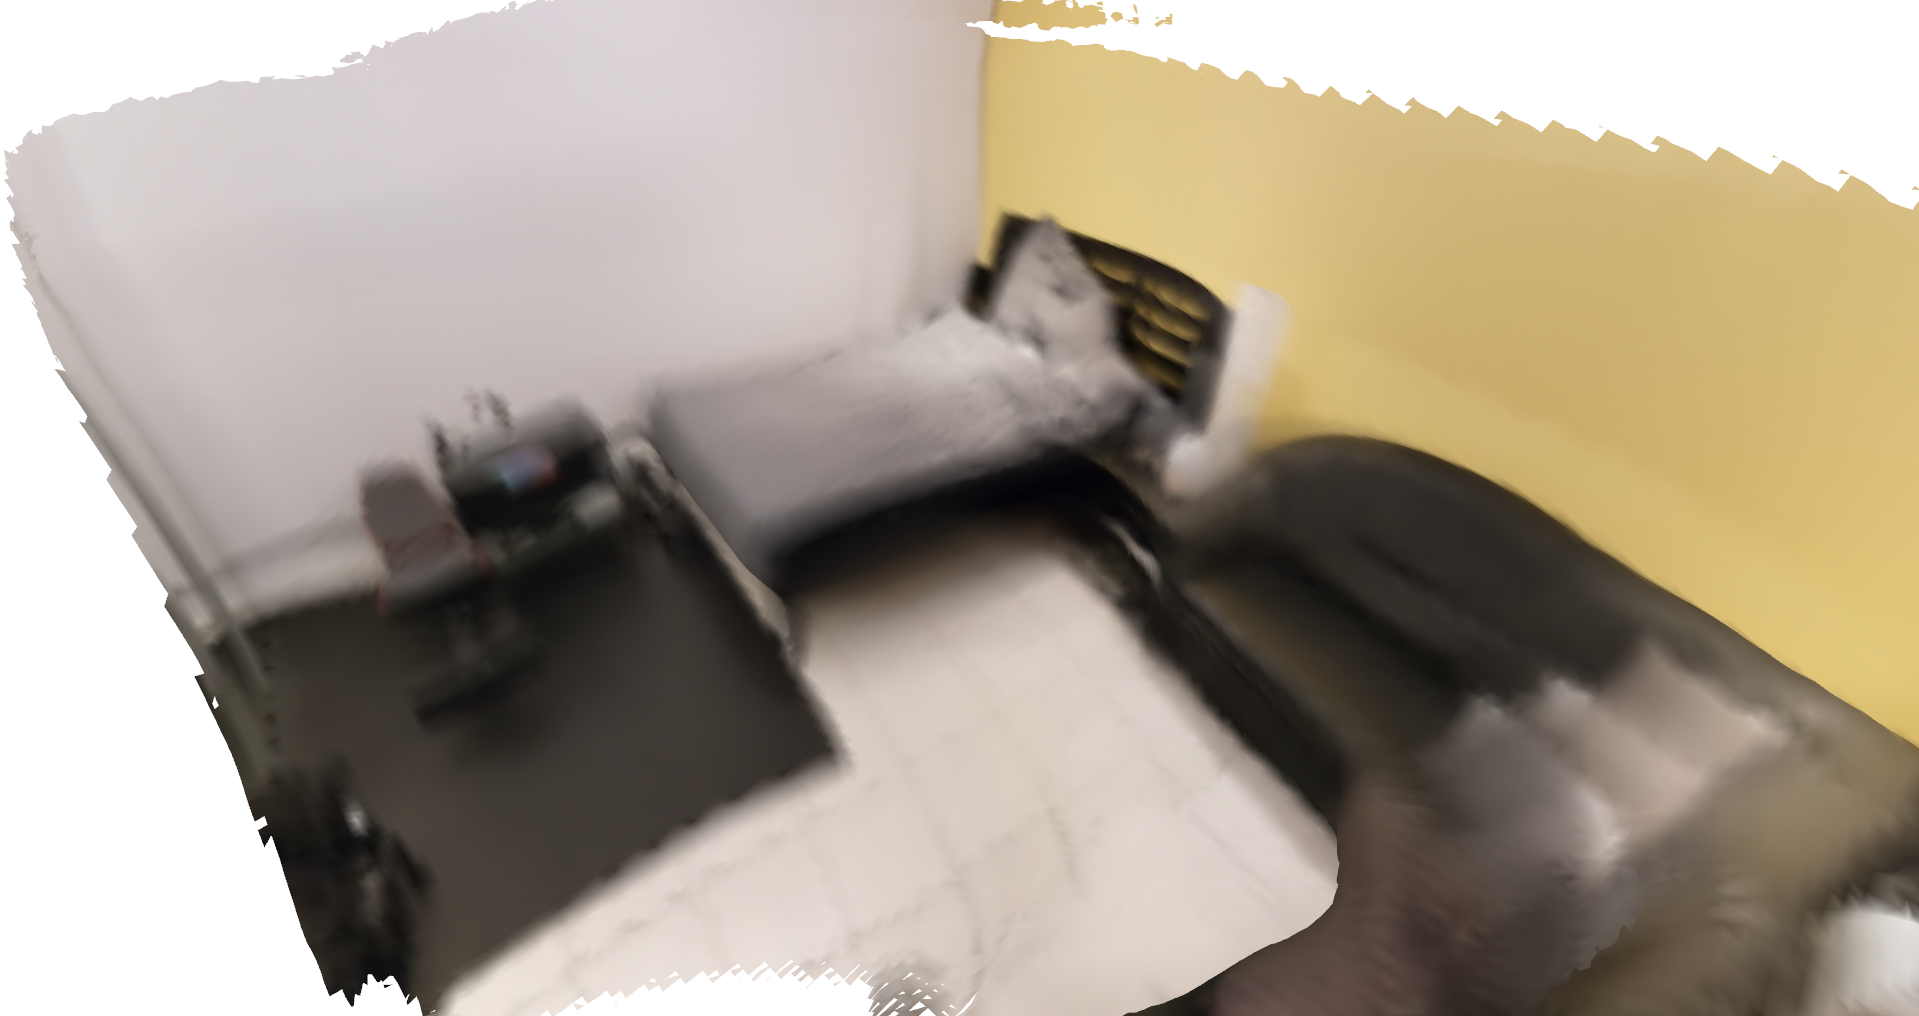
\includegraphics[width=.6\textwidth]{images/initial_reconstruction.png}
            \caption{Initial reconstruction on unoptimized pose estimates on one of our own videos.}
            \label{fig:initial_reconstruction}
        \end{figure}
        It turned out that our method for the pose estimation, described in chapter~\ref{sec:method_pose_optimization}, while not meant to be fast, was actually very computationally expensive.
        As the amount of frames increases, the number of valid frame pairs can potentially grow exponentially.
        In order to avoid computing for unreasonable amounts of time, we used a similar method to reduce the computational effort as described in \citetitle{dai2017bundlefusion}~\cite{dai2017bundlefusion}.
        While They use a hierarchy to condense the information within one chunk of 11 frames into one keyframe, we simply selected our keyframes without using the information of the remaining frames.\\
        As we could not identify a visible improvement after the pose optimization, we ran everything on the synthetic dataset 'lr kt2' from \citetitle{handa:etal:ICRA2014}~\cite{handa:etal:ICRA2014}.
        With the ground truth of the extrinsics we were able to properly compare our initial poses to the optimized poses.
        To compare extrinsics from different coordinate systems we needed to find a transform to match the trajectories.
        This transform includes rotation, scaling, and translation.
        One option is to simply align the poses of the first frame.
        While this is a trivial method, it does not lead to a satisfying alignment and makes it really hard to find the proper scale.
        Results of this alignment are shown in figure~\ref{sfig:align_first_pair}.\\
        We can observe that the alignment is not satisfactory.
        Employing a method like ICP (iterative closest point) achieves a much better alignment.
        We implemented an error function for the deviation of the two trajectories that takes 7 unknowns: three angles for the rotation $R$, three variables for the translation $t$, and one unknown for the scale $s$:
        \begin{equation*}
            E_{\text{alignment}}(R,t,s) =
            \sum_{i=0} \left[
                q_i - s \times Rp_i - t
            \right]^2
            \label{eq:ealign}
        \end{equation*}
        Where $q_i$ is point $i$ of the target trajectory and $p_i$ is point $i$ of the trajectory that is transformed.
        With this error function we again used scipy.optimize.minimize to obtain the optimal transform.
        The results are displayed in figures~\ref{sfig:align_global}~\&~\ref{sfig:align_global_opt}\\
        \begin{figure}[ht]
            \centering
            \begin{subfigure}[b]{.32\textwidth}
                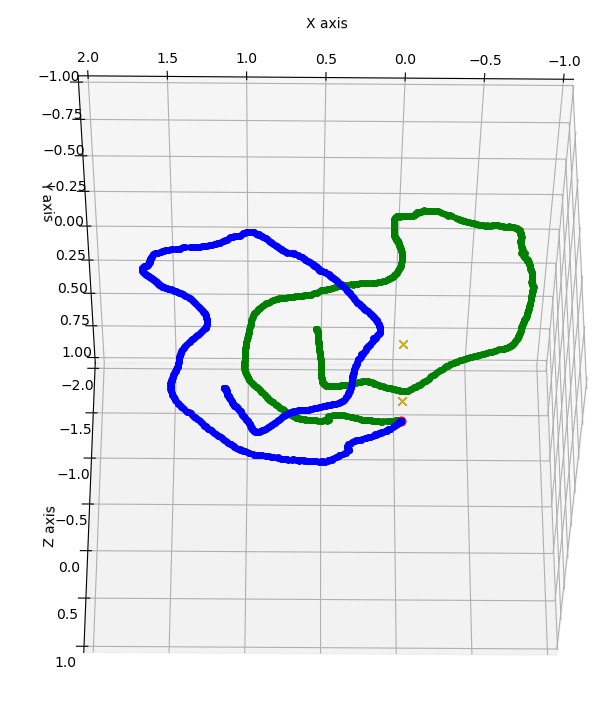
\includegraphics[width=.95\textwidth]{images/align_first_pair}
                \caption{Aligning two trajectories by aligning the first pose of both.}
                \label{sfig:align_first_pair}
            \end{subfigure}
            \begin{subfigure}[b]{.32\textwidth}
                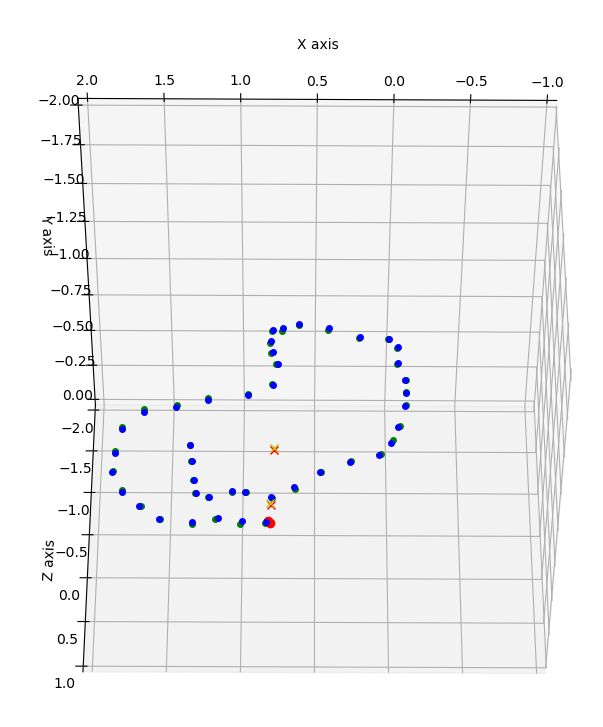
\includegraphics[width=.95\textwidth]{images/align_global}
                \caption{ICP-like global alignment of unoptimized extrinsics}
                \label{sfig:align_global}
            \end{subfigure}
            \begin{subfigure}[b]{.32\textwidth}
                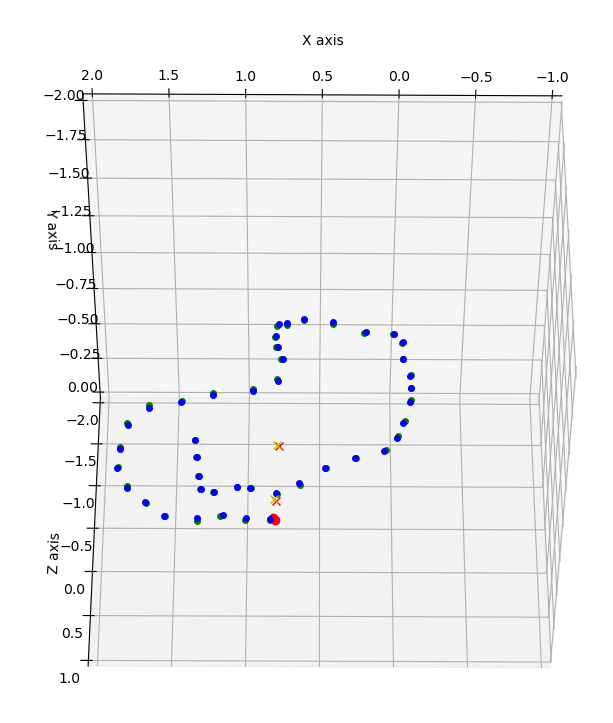
\includegraphics[width=.95\textwidth]{images/align_global_opt}
                \caption{ICP-like global alignment of optimized extrinsics}
                \label{sfig:align_global_opt}
            \end{subfigure}
            \caption[]{\ref{sfig:align_first_pair} aligning both initial poses perfectly. \ref{sfig:align_global} ICP-like global alignment of unoptimized extrinsics. \ref{sfig:align_global_opt} ICP-like global alignment of optimized extrinsics. For both trajectories the orientation of the first pose is indicated by two crosses into the direction the camera is facing, red for ground truth and yellow for the other trajectory. \ref{sfig:align_global}~\&~\ref{sfig:align_global_opt} were reduced with a stride of 20.}
            \label{fig:vis_perspective}
        \end{figure}
        While the cost function described in equation~\ref{eq:edense} provides a lower cost for the optimized extrinsics, the alignment error from equation~\ref{eq:ealign} was actually higher than the unoptimized extrinsics.
        So the optimized poses actually fir worse to the ground truth than the initial estimates:
        \begin{center}
            \begin{tabular}[]{c | c | c}
                & unoptimized poses & optimized poses\\
                \hline
                $E_{\text{dense}}$ & $1.7203$ & $1.6081$\\
                \hline
                $E_{\text{alignment}}$ & $1.2420\times10^{-2}$ & $1.2998\times10^{-2}$
            \end{tabular}
        \end{center}
        As the optimized extrinsics also showed little to no improvement to the 3D reconstruction we analyzed the quality of our depth estimates.
    \section{Consistent Depth}
        \begin{itemize}
            \item maybe lead with a screenshot from the 3D reconstruction and a relevant frame from the video that shows, that corners are rounded and the depth is obviously flawed! (protein-tuete, ecken, meine wand die auch omegarund ist)
            \item describe how we compared the "consistent depth depth" to the ground truth --> leads to error heatmap that shows how off the depth estimate is
        \end{itemize}

  \chapter{Conclusion}
    \todo{our pose optimization can't improve the extrinsics when it is so heavily based on the depth that is so shit..}
    conclusion may be, that the optimization just requires all the things we skipped.. better solver, better jacobian, better outlier filtering, ..\\
    or that the depth is just a bit fucked and the optimization approach actually works with the ground truth depth
    \begin{itemize}
        \item option1: blame everything on shitty depth (arguing, that the optimizer did the best he could) [I VOTE FOR THIS OPTION]
        \item option2: possibly present magical scale fix [I DONT SEE HOW THIS OPTION COULD STILL BE RELEVANT]
        \item option3: depth is not at fault and our optimization is just sadly not working as we want it to [THIS IS PROBABLY KINDA TRUE]
    \end{itemize}
    we probably end up with a combination of option 1 and 3\\
    maybe we should point out, that we may have underestimated the effort required for this project? (or not.. idk)\\
    what we sadly did not have enough time for, was to attempt the extrinsics refinement with the true depth and normals that are based on the true depth. this would show us if the optimization in itself works or not. the current results point to the refinement making the extrinsics worse. but that could very well be because of the broken depth that is used in the refinement process!\\
    optimization could have been improved with masks from FlowNet\\

% This ensures that the subsequent sections are being included as root
% items in the bookmark structure of your PDF reader.
\bookmarksetup{startatroot}
\backmatter

	\begingroup
		\let\clearpage\relax
		\glsaddall
		% \printglossary[type=\acronymtype]
		% \newpage
		\printglossary
		% \newpage
		% \listoffigures
	\endgroup

	\printindex
	\printbibliography

\end{document}
